\section*{Chapter~4~~Research~Solution}
\setcounter{section}{4} \setcounter{subsection}{0} 
\setcounter{table}{0} \setcounter{figure}{0} \setcounter{equation}{0}\setcounter{definition}{0}
\addcontentsline{toc}{section}{\textbf{Chapter~4~~Research~Solution}}

\subsection{Environment Setup}
% Experiment Settings
\noindent In this section, we will detail the construction of BLE network testbed, as well as comprehensive information regarding the deployment environment and the devices involved. To ensure the reliability and reproducibility of the experiments, all hardware devices and software platforms utilized are readily accessible and well-documented on the Internet.

\subsubsection{Testbed Implementation}

\noindent In a word, the testbed environment can be categorized into four parts: (i) BLE devices, (ii) user devices, (iii) attacker platforms, and (iv) network sniffers. \textbf{Table 4-1} comprehensively illustrates all the components utilized in the network testbed.

\begin{table}[H]
    \centering
    \caption{Components of proposed BLE network testbed.}
    % \tabcolsep=0.5cm
    \renewcommand\arraystretch{1.2}
    
    \resizebox{\textwidth}{!}{
    \begin{tabular}{ccc} 
    \toprule[1.2pt]
        \textbf{Component} & \textbf{Description} & \textbf{Devices Example} \\ \midrule
        BLE devices & Used to build the BLE cyberspace environment & nRF51822, DA14580 chips \\
        User devices & Used to connect and simulate usage scenarios & Apple laptop, Android phone \\
        Attacker platforms & Used to launch advanced spoofing attacks & CSR dongle, Lenovo laptop \\
        Network sniffers & Used to capture network advertising package & Raspberry Pi, BLE-Analyzer \\
        \bottomrule[1.2pt]
    \end{tabular}
    \label{tab-4-1}
    }
\end{table}

\subsubsection{Deployment Environment}
\noindent The testbed was strategically deployed within a physical environment: a $15m \times 15m$ office space configured with 18 cubicles, as illustrated in \textbf{Figure 4-1}. The office was methodically partitioned into $1m \times 1m$ grids. This setting typifies a complex and acoustically active indoor environment, presenting significant challenges for evaluating the detection efficiency of BLEGuard. During data collection, RF signals were monitored within the range of our sniffers, uncovering considerable channel interference. This interference was primarily caused by 40 devices equipped with Bluetooth or BLE technologies, including smartphones, speakers, mice, and keyboards, along with numerous Wi-Fi access points and two microwave ovens. It was also noted that the sudden movements of individuals within the office substantially affected the channel conditions, further complicating the monitoring environment.

\subsubsection{BLE Devices}
\noindent For the construction of our network testbed, we utilized sixteen commonly used BLE devices featuring a range of Bluetooth chips, including nRF51822 and DA14580, as catalogued in \textbf{Table 4-2}. After evaluating their performance, we selected nine devices that demonstrated consistent stability, suitable for our data collection needs. These devices represent a wide array of typical BLE applications, providing a comprehensive overview of potential real-world uses.

\begin{figure}[h]
    \centering
    \caption*{Table 4-2 BLE devices used in proposed network testbed.}
    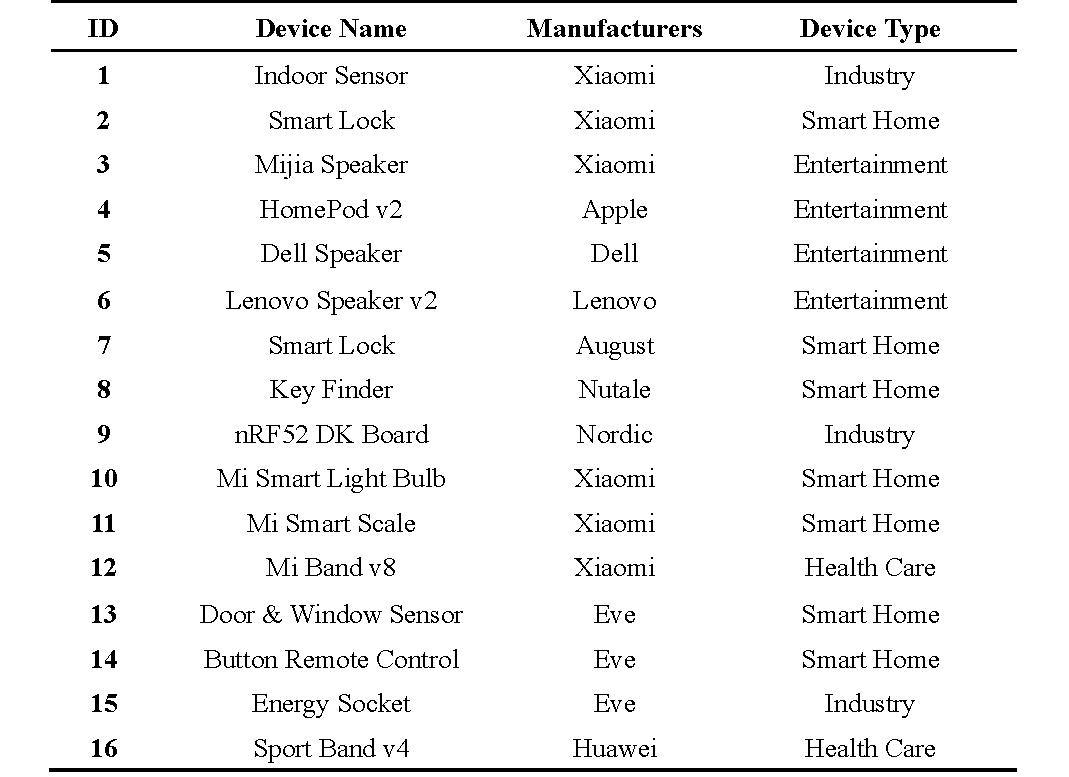
\includegraphics[width=0.96\linewidth]{FZU thesis templete//Table/appendices-1-1.pdf}
\end{figure}

\subsubsection{User Devices}
% \noindent The user devices are used to connect with BLE devices to simulate network scenarios under normal usage. We also implemented the monitor on the user laptop and PC to interact with sniffers and receive the datasets. \textbf{Table 4-3} illustrates the user devices utilized in our network environment. Besides, it was mentioned above that we have about 40 other network devices in our deployment office, but we only collect the network datasets from the BLE devices we deployed, and we do not record any data from other unknown devices.

\noindent In our testbed, user devices are employed to connect with BLE devices, simulating typical network scenarios. Monitoring software has been implemented on user laptops and PCs to facilitate interaction with network sniffers and to collect datasets. \textbf{Table 4-3} details the user devices employed within our network environment. Additionally, while approximately 40 other network devices are present in our deployment office, data collection is exclusively focused on the BLE devices we specifically deployed, with no data recorded from any unidentified devices.

\subsubsection{Attacker Platforms}
\noindent To generate multiple spoofing attacks, we deployed four distinct types of attacker platforms, each comprising three identical samples situated at different locations. The specifics of the attacker platforms used in our testbed are outlined in \textbf{Table 4-4}. We opted for these platforms due to their accessibility, programmability, and utilization of various transmit power values \cite{yaseen2019marc}. In addition, we provided the MAC address for each device to distinguish between identical devices performing different functions, since we have multiple duplicate copies.

\subsubsection{Network Sniffers}
\noindent Within the office environment, three network sniffers were precisely positioned at predetermined grid coordinates, each powered by a Raspberry Pi running BLE-Analyzer-PRO software. This adaptable platform, suitable for further development, enabled the detailed capture of network packets and their cyber-physical features. The Raspberry Pi also managed the transmission of the collated datasets to the monitoring systems. The total cost of this sniffer configuration was approximately 80 dollars, demonstrating a budget-friendly approach to comprehensive network monitoring. For a more in-depth overview of the sniffer equipment used, refer to \textbf{Appendices 1}.

\vspace{4pt}

\begin{figure}[h]
    \centering
    \caption*{Table 4-3 User devices used in BLEGuard testbed.}
    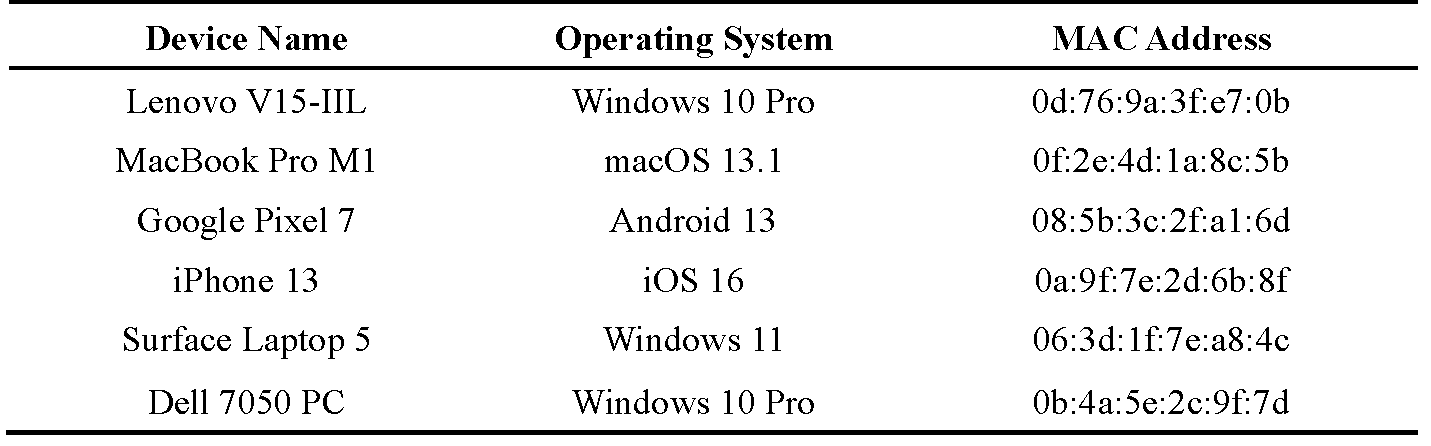
\includegraphics[width=0.92\linewidth]{FZU thesis templete//Table/appendices-1-2.pdf}
\end{figure}


\begin{figure}[h]
    \centering
    \caption*{Table 4-4 Attacker platform used in BLEGuard testbed.}
    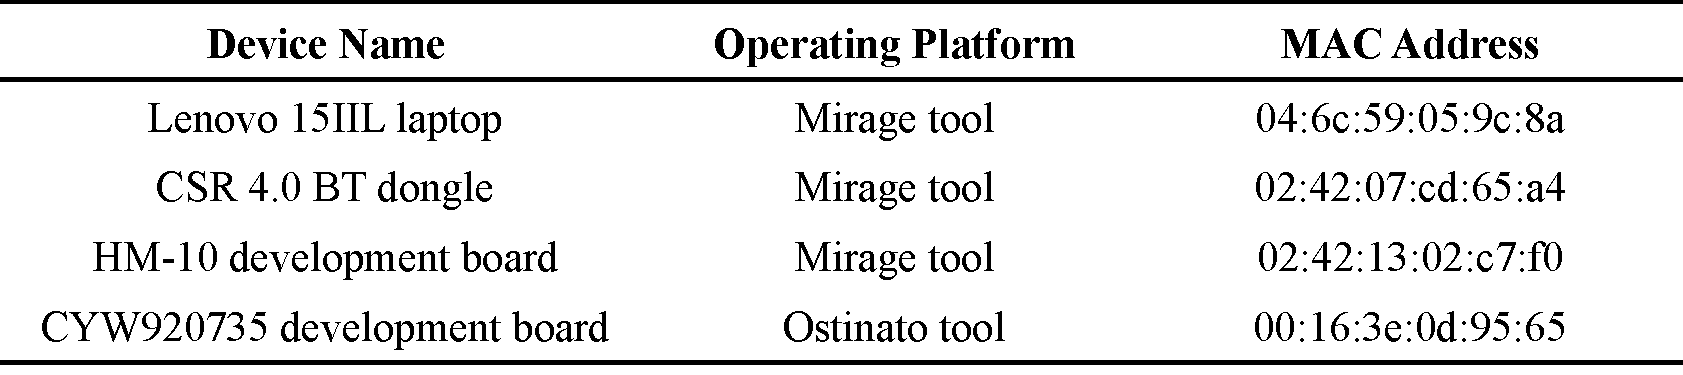
\includegraphics[width=0.92\linewidth]{FZU thesis templete//Table/appendices-1-3.pdf}
\end{figure}

\vspace{4pt}

% ————————————————————————————————————————————————————————————————————— %
% ————————————————————————————————————————————————————————————————————— %
% ————————————————————————————————————————————————————————————————————— %
% ————————————————————————————————————————————————————————————————————— %


\subsection{Data Preparation}

\noindent This section delineates the procedures for implementing the network testbed, simulating spoofing attacks, and constructing network datasets. To ensure the reliability and reproducibility of our experiments, we will make both our data and the associated code publicly accessible \cite{EasyChair:10902}.

\subsubsection{Attack Simulation}
\noindent As mentioned above, the BLEGuard system was operationalized within the testbed using user monitoring devices and network sniffers. These devices collaborated to manage the collection of network datasets, utilizing the Wireshark tool to analyze traffic. The coordination of network activities, from communication between monitors and sniffers to the exchange of advertising packets and gathering of cyber-physical features, was handled by a Python script comprising approximately 2000 lines of code. This principal script is included in the supplementary materials.

\subsubsection{Data Pre-processing}
\noindent As outlined in \textbf{Table 4-4}, four types of attacker platforms were strategically deployed, with three units of each type, across twelve distinct locations. This setup enriched the cyber-physical feature datasets, particularly for RSSI and CFO. \textbf{Figure 4-1} visually represents this arrangement within the testbed environment, where sixteen BLE devices are marked by blue circles, six sniffers by green squares, and twelve attacker platforms by red triangles. In the simulated attack scenarios, identity information was cloned using USB dongles, the Mirage tool \cite{sun2020towards}, and the Ostinato tool \cite{khamaiseh2019detecting} to disrupt normal network connections between BLE devices and user devices. This experiment underscores the ease with which advanced attackers could exploit vulnerabilities in BLE to manipulate device settings, posing significant security risks.


\begin{figure} %[H]
    \centering
    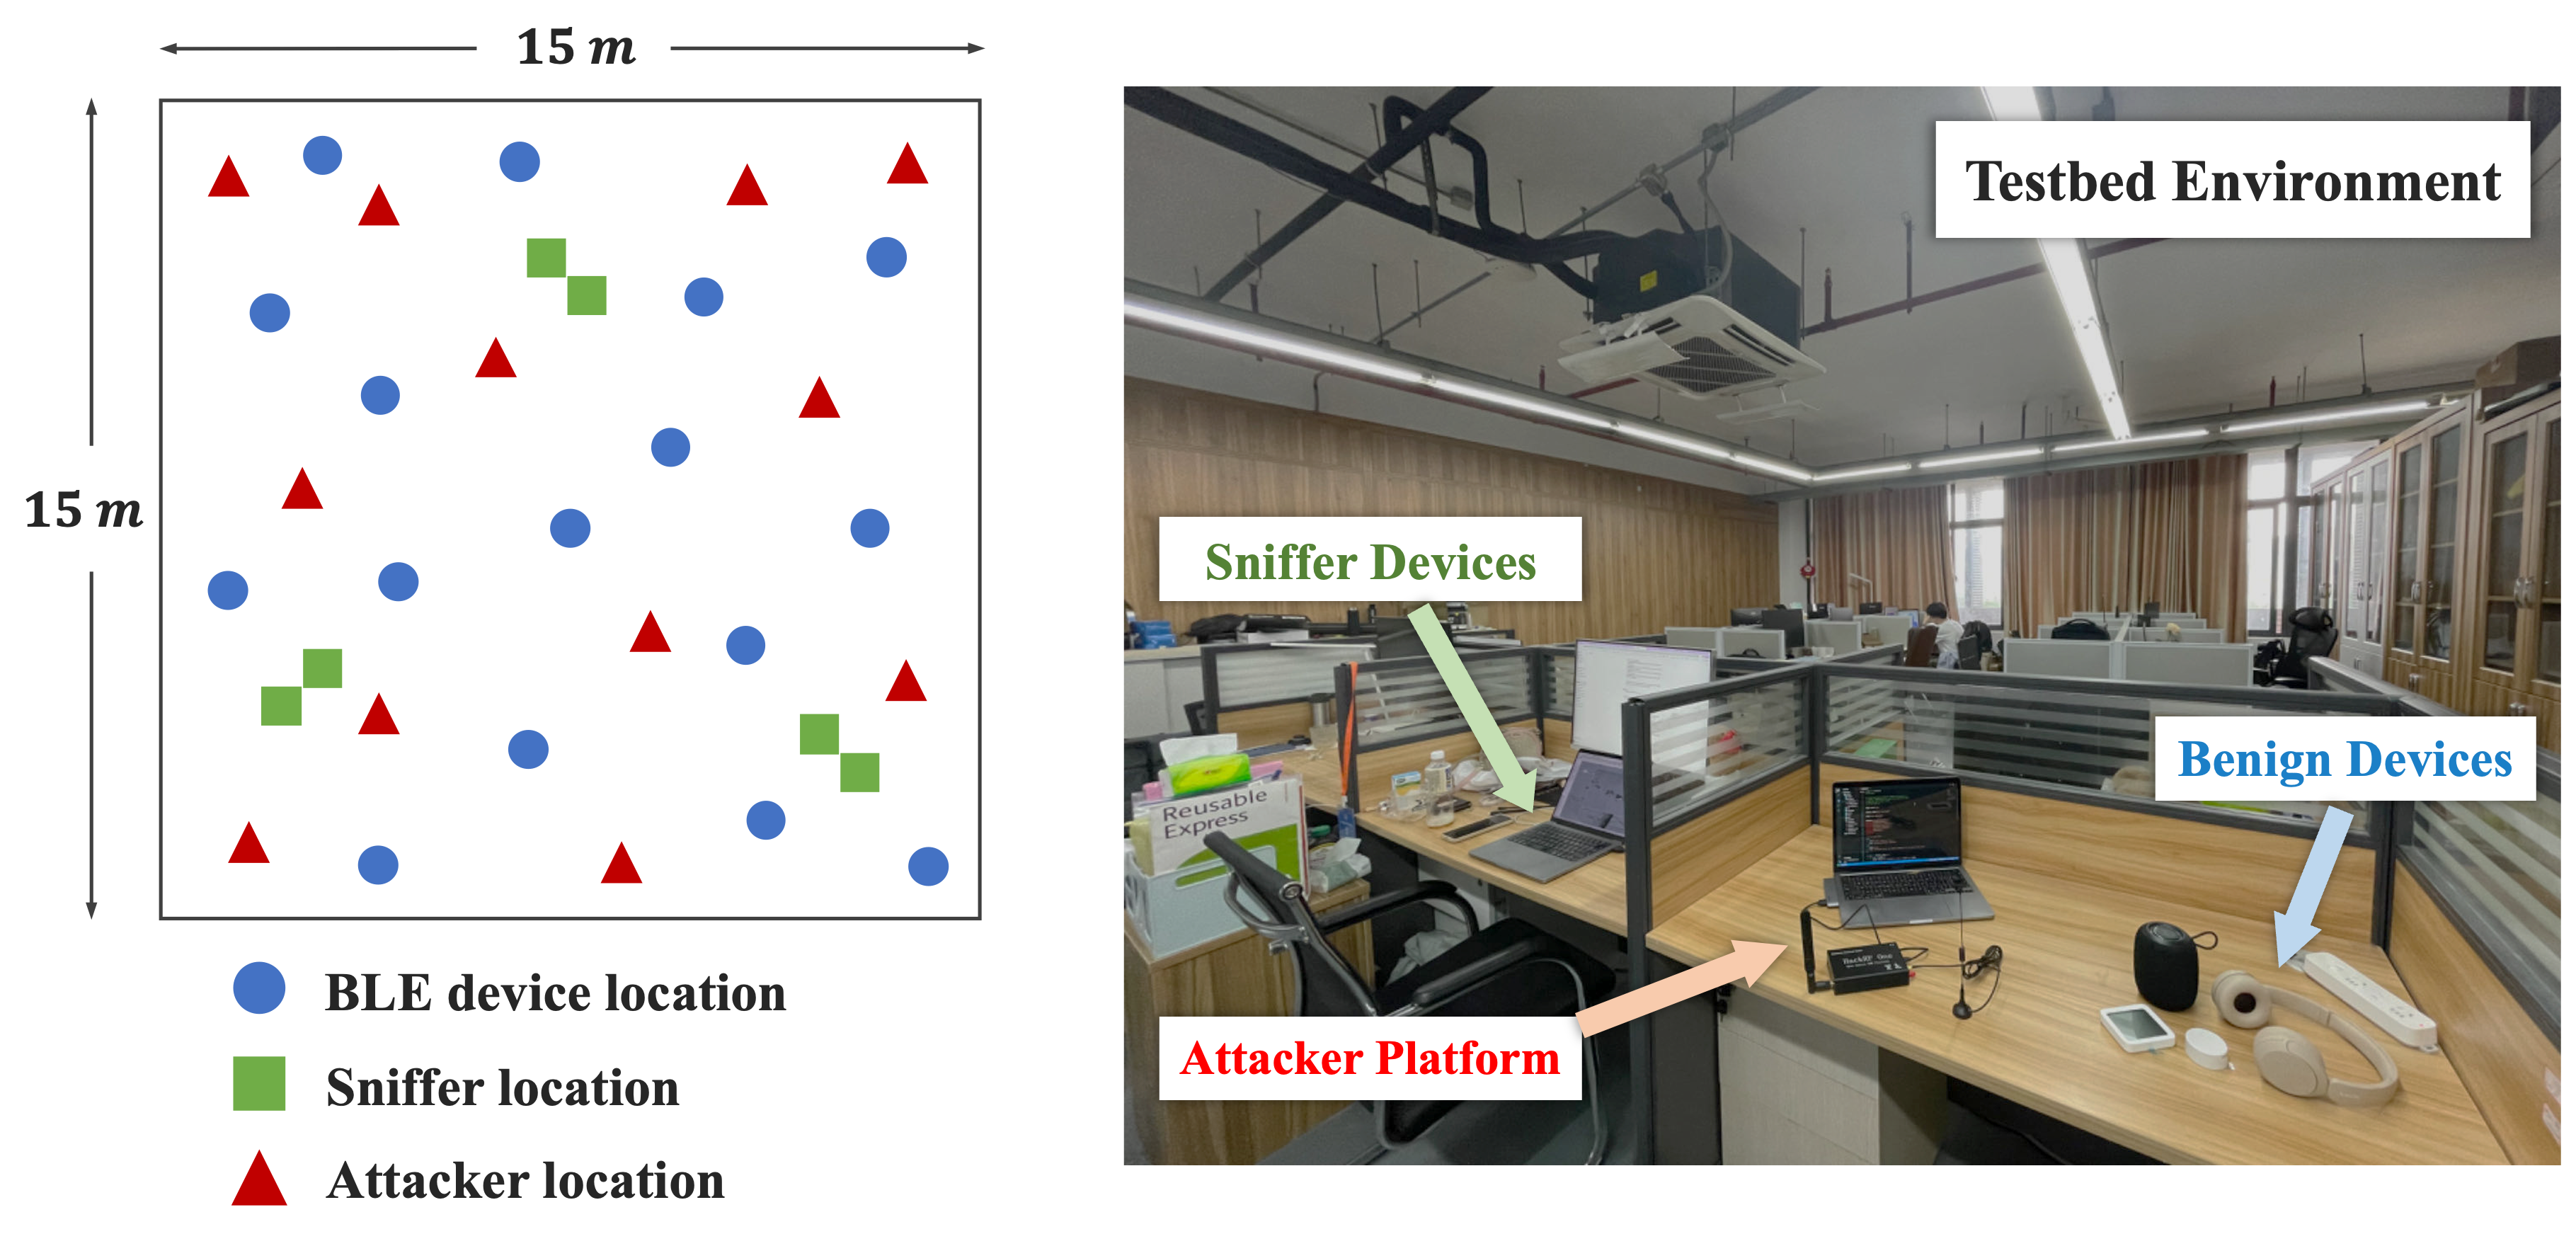
\includegraphics[width=1\linewidth]{FZU thesis templete//Fig/fig4-1.png}
    \caption{Locations of three types of devices in BLEGuard testbed.}
    \label{fig-4-1}
    \vspace{6pt}
\end{figure}

\vspace{6pt}

\subsubsection{Datasets Building}

\noindent Regarding the building of our dataset, we meticulously collected normal advertising packets from each BLE device over a period of approximately eight hours—five hours during daytime and three hours at nighttime. Additionally, for each attacker platform situated in various positions, malicious packets were collected for about 20 minutes. Currently, our BLE Spoofing Attack Dataset (\textit{BLE-SAD}) contains 906,000 advertising packets, of which 81.6\% are benign and 18.4\% are malicious. The open-source dataset can be accessed at: \href{https://github.com/BLEGuard/supplement}{https://github.com/BLEGuard/supplement}.

\vspace{32pt}

% ————————————————————————————————————————————————————————————————————— %
% ————————————————————————————————————————————————————————————————————— %
% ————————————————————————————————————————————————————————————————————— %
% ————————————————————————————————————————————————————————————————————— %


\subsection{Detection Mechanism}
\noindent In this section, we will discuss our proposed BLEGuard system, a hybrid detection mechanism combined cyber-physical analysis with machine learning techniques.


\subsubsection{Pre-detection Scheme}

\noindent In BLEGuard, suspicious activities are identified through the detection of atypical fluctuations in cyber-physical features such as Used Channel Numbers (UCN), Advertising Interval (INT), Carrier Frequency Offset (CFO), and Received Signal Strength Indicator (RSSI). Abrupt changes in UCN and INT may indicate potential security threats, while RSSI and CFO are crucial for a continuous pre-detection mechanism that anticipates advanced spoofing attacks.

\vspace{8pt}

To effectively monitor these indicators, BLEGuard employs three network sniffers that capture the values of these features within a \textit{lookback window}. The lookback window refers to a predefined period prior to the current analysis point, during which data is collected to establish a baseline for normal behavior. This historical data is essential for understanding typical network conditions and variations. Subsequently, the system evaluates the current network activity by examining the values from an \textit{observation window}, which is the period immediately following the lookback window. This approach allows BLEGuard to compare present data against the baseline to spot any irregularities or deviations.

\vspace{8pt}


An alarm is triggered if there are deviations from the established norms in any of the monitored features, indicating a potential security breach. This method can be seamlessly integrated into existing BLE networks without causing disruption or significant resource consumption. Detailed detection schemes for each feature are outlined as follows:

\vspace{8pt}

\noindent \textbf{$\bullet$ Metric 1: Used Channel Numbers}

\noindent In BLE networks, Used Channel Numbers (UCN) designates the sequence of radio channels that BLE devices utilize for transmission, adhering to a preconfigured pattern to enhance connectivity and reduce noise interference. The stability of UCN patterns can be compromised during spoofing attacks, as attackers may instigate an irregular shift in the communication channels, thus disrupting the network's harmonious channel utilization. To quantify such fluctuations, we introduce the metric \( UCN_{\text{change}} \), which represents the cumulative measure of channel switching activity:

\vspace{-4pt}

\begin{equation}
UCN_{\text{change}} = \sum_{i=1}^{N_{\text{obs}}} \left| UCN_i - UCN_{i-1} \right|,
\end{equation}

where \( N_{\text{obs}} \) is the count of observed transmission packets and \( UCN_i \) corresponds to the utilized channel for the \( i^{th} \) packet transmission. An elevated \( UCN_{\text{change}} \) value is indicative of more frequent channel alternations, potentially signaling an ongoing spoofing attack. For operational integrity in BLE networks, an acceptable threshold for \( UCN_{\text{change}} \), denoted by \( \Delta UCN_{\text{normal}} \), is set at 2.8. This threshold indicates the maximum allowable frequency of channel changes within a defined observation period. A breach of this threshold is symptomatic of anomalous behavior:

\vspace{-4pt}

\begin{equation}
\text{If } UCN_{\text{change}} > \Delta UCN_{\text{normal}}, \text{ then activate further detection.}
\end{equation}

Employing \( UCN_{\text{change}} \) as a heuristic enables a robust security framework capable of detecting and responding to potential spoofing threats, thereby fortifying the BLE network's defenses.

\vspace{6pt}

\noindent \textbf{$\bullet$ Metric 2: Advertising Interval}

\noindent The Advertising Interval (INT) is also a key parameter in BLE communications, defining the time gap between consecutive advertising packets. This interval is crucial for maintaining the orderly transmission of broadcast information in BLE networks. By definition, the INT between any two consecutive advertising packets should never fall below a predefined lower bound, which is set based on the specifications of the BLE device and the operational requirements of the network. This lower bound is denoted as $L_{\text{int}}$. The formula used to compute the runtime INT value, $INT$, for the interval between two packets is given by:

\vspace{-4pt}

\begin{equation}
INT = T_{\text{current}} - T_{\text{previous}}
\end{equation}

where $T_{\text{current}}$ is the timestamp of the current advertising packet, and $T_{\text{previous}}$ is the timestamp of the immediately preceding advertising packet. The Advertising Interval (INT) is calculated as the difference between these two timestamps. If \(INT\) is found to be less than the predefined lower limit \(L_{\text{int}}\), the monitor identifies this condition as anomalous. Such a scenario indicates a potential operational fault or a security breach, such as a spoofing attack that attempts to flood the network with frequent, unauthorized advertising packets. Upon detecting such an anomaly, the monitor triggers an alarm, alerting the system to the potential threat. Typically, \(L_{\text{int}}\) is set to a threshold value of 10 milliseconds to detect rapid, unscheduled transmissions \cite{wu2020blueshield}. The corresponding condition can be mathematically expressed as:

\vspace{-4pt}

\begin{equation}
\text{If } INT < L_{\text{int}}, \text{ then activate further detection.}
\end{equation}

This monitoring mechanism ensures the integrity and correct functioning of the BLE network by verifying that the advertising packets are transmitted within the expected intervals, adhering to the designed operational parameters.

\vspace{6pt}

\noindent \textbf{$\bullet$ Metric 3: CFO level}

\noindent BLEGuard continuously monitors the CFO (Carrier Frequency Offset) and RSSI (Received Signal Strength Indicator) values from advertising packets. Upon activation of the CFO and RSSI inspection, BLEGuard analyzes these values through the following procedure. For a BLE device exhibiting intermittent advertising patterns, we define the lookback window as the time period $T_l$ (with $N_l$ packets) before the transition from advertising to connection state, and the observation window as the time period $T_o$ (with $N_o$ packets) after the transition from connection back to advertising state. In BLEGuard, following the reception of a connection request packet, the monitoring system initiates the CFO and RSSI inspections for advertising packets collected from each device across the three advertising channels (37, 38 and 39). The system first calculates the acceptable ranges for CFO and RSSI values using data from the lookback window. It then evaluates these metrics in the advertising packets during the observation window. If an anomaly is detected in either the CFO or RSSI readings, an alarm is triggered.

\vspace{6pt}

The CFO values observed from BLE networks are expected to conform to a Gaussian distribution \cite{wu2020blueshield}. Consequently, when $ \mu_{0} $ and $ \sigma_{0} $ represent the mean and standard deviation of these CFO values, the probability distribution function for the CFO can be articulated as:

\vspace{-4pt}

\begin{equation}
F_{cfo}(x_i) = \frac{1}{\sigma_{0} \sqrt{2\pi}} \cdot e^{-\frac{\left(x_i-\mu_0\right)^2}{2 \sigma_0^2}}
\end{equation}

where $ x_i $ denotes a sample CFO value. In BLEGuard, the monitor employs the CFO values from advertising packets within a lookback window, comprising $ N_l $ packets, to calculate $ \mu_{0} $ and $ \sigma_{0} $. These parameters are then integrated into the probability function previously mentioned. If the advertising packets from both the lookback and subsequent observation windows originate from the same BLE device, the CFO values from the observation window's advertising packets should statistically align with the given distribution. This is verified by the monitoring system calculating the negative log-likelihood of the CFO values from the observation window packets, defined as:

\vspace{-4pt}

\begin{equation}
L_{cfo} = \frac{1}{N_o} \sum_{i=1}^{N_o} -\log F_{cfo}(x_i)
\end{equation}

If the log-likelihood value is less than a predetermined CFO inspection threshold, denoted by $ \beta_{cfo} $ (i.e., $ L_{cfo} < \beta_{cfo} $), the CFO values are considered to be within the normal range for the BLE device. This threshold $ \beta_{cfo} $ is a tunable parameter within BLEGuard that dictates the permissible range of CFO values during the observation window. In contrast, if the log-likelihood value exceeds $ \beta_{cfo} $ (i.e., $ L_{cfo} > \beta_{cfo} $), an anomaly is recognized, and an alarm is activated, signaling a possible spoofing attack. In most real-world scenarios, $\beta_{cfo}$ is generally set to 3.

\vspace{6pt}

\noindent \textbf{$\bullet$ Metric 4: RSSI level}

\noindent To detect anomalies in RSSI values amid strong signal reflections in BLE networks, we utilize a two-component Gaussian mixture model. This approach is chosen because RSSI values in environments with high noise can be effectively modeled using two normal distributions \cite{sheng2008detecting}. The probability distribution function for RSSI values is given by:

\vspace{-4pt}

\begin{equation}
\label{eq4-1}
F_{rssi}\left(y_i\right)=w \cdot \frac{1}{\sigma_1 \sqrt{2 \pi}} \cdot e^{-\frac{\left(y_i-\mu_1\right)^2}{2 \sigma_1^2}}+(1-w) \cdot \frac{1}{\sigma_2 \sqrt{2 \pi}} \cdot e^{-\frac{\left(y_i-\mu_2\right)^2}{2 \sigma_2^2}}
\end{equation}

In this equation, $\mu_1$ and $\mu_2$ are the means of the two components, $\sigma_1$ and $\sigma_2$ are their standard deviations, $w$ is a weight parameter that balances the two components, and $y_i$ is an RSSI sample. Using the BLEGuard system, $N_l$ of RSSI values from advertising packets within a lookback window are analyzed to estimate the parameters $\mu_1, \mu_2, \sigma_1, \sigma_2$, and $w$ through a conventional expectation-maximization (EM) algorithm \cite{guo2018expectation}. Following this, the monitor calculates the negative log-likelihood that the RSSI values $\left(y_i, \forall i \in\left[1, N_o\right]\right)$ from the observation window conform to the model specified by Equation (4-7):

\vspace{-4pt}

\begin{equation}
\label{eq4-2}
L_{rssi}=\frac{1}{N_o} \sum_{i=1}^{N_o}-\log F_{rssi}\left(y_i\right)
\end{equation}

% An anomaly is detected if this negative log-likelihood exceeds a predefined RSSI inspection threshold, $\delta_{rssi}$ (i.e., $L_{rssi}>\delta_{rssi}$). The threshold $\delta_{rssi}$ is a critical design parameter in BLEGuard, set to optimize detection sensitivity and specificity (usually define $\delta_{rssi }=5$).

An anomaly is detected when the negative log-likelihood surpasses a predefined RSSI inspection threshold, denoted as $\delta_{\text{rssi}}$ (i.e., $L_{\text{rssi}} > \delta_{\text{rssi}}$). The threshold $\delta_{\text{rssi}}$ is a crucial parameter in BLEGuard, calibrated to optimize detection sensitivity and specificity. Typically, $\delta_{\text{rssi}}$ is set to 5.


% ————————————————————————————————————————————————————————————————————— %
% ————————————————————————————————————————————————————————————————————— %


\subsubsection{Reconstruction Model}
% \noindent Upon detecting suspicious activities, we embark on a comprehensive analysis of anomalous data batches. A Temporal Convolutional Network (TCN) \cite{lea2017temporal} is utilized to reconstruct traffic patterns, facilitating the isolation of aberrant data through comparative analysis. During the offline training phase, our aim is to minimize the error between the learned data $D_L$ and the original dataset $D_T$. In the online testing phase, the presence of malicious packets in the input data leads to an increase in the reconstruction error. The residual is defined as $R(D_T, D_L) = |D_T - D_L|$ with $D_L = f(D_T)$, where $f$ denotes the transformation function of the TCN auto-encoder. We assess this residual to determine the anomaly score $\alpha$ for each data batch, as depicted in Equation (1), with $R_\alpha$ representing the corresponding residual, $\mu$ as the mean value of the residual, and $\sigma$ as its standard deviation.

\noindent Upon identifying suspicious activities, a thorough analysis is initiated on anomalous data batches. To facilitate this, a Temporal Convolutional Network (TCN) \cite{lea2017temporal}, as illustrated in \textbf{Figure 4-2}, is employed to reconstruct traffic patterns. This approach helps isolate aberrant data through comparative analysis. A TCN is a type of neural network specifically designed for sequence modeling that combines convolutional layers with causal connections to ensure that predictions for a specific time step can only depend on past data. This structure makes TCNs particularly effective for time series predictions where past context is crucial.

\vspace{8pt}

During the offline training phase, the objective is to minimize the discrepancy between the learned data $D_L$ and the original dataset $D_T$. In the online testing phase, the presence of malicious packets in the input data triggers an increase in the reconstruction error, indicative of potential spoofing threats. The residual, defined as $R(D_T, D_L) = |D_T - D_L|$ with $D_L = f(D_T)$, where $f$ represents the transformation function employed by the TCN auto-encoder, serves as a critical metric. This residual is assessed to calculate the anomaly score $\alpha$ for each data batch, as depicted in Equation (4-9). Here, $R_\alpha$ denotes the calculated residual, $\mu$ is the mean value of the residual, and $\sigma$ is its standard deviation. \textbf{Figure 4-2} demonstrates how benign inputs lead to benign outputs, whereas malicious inputs result in malicious outputs, showing the operational mechanism of TCN.



% \vspace{-2pt}

\begin{equation}
\label{eq4-3}
\alpha=\left\{\begin{array}{l} 
0, \text ~{when}~ \left|R_\alpha-\mu R_\alpha\right| \leq 3 * \sigma R_\alpha~\to~{Normal~Data~Batch} \\
1, \text ~{when}~ \left|R_\alpha-\mu R_\alpha\right| \textgreater 3*\sigma R_\alpha~\to~{Suspicious~Data~Batch}
\end{array}\right.
\end{equation}

\vspace{6pt}

\begin{figure}%[H]
    \centering
    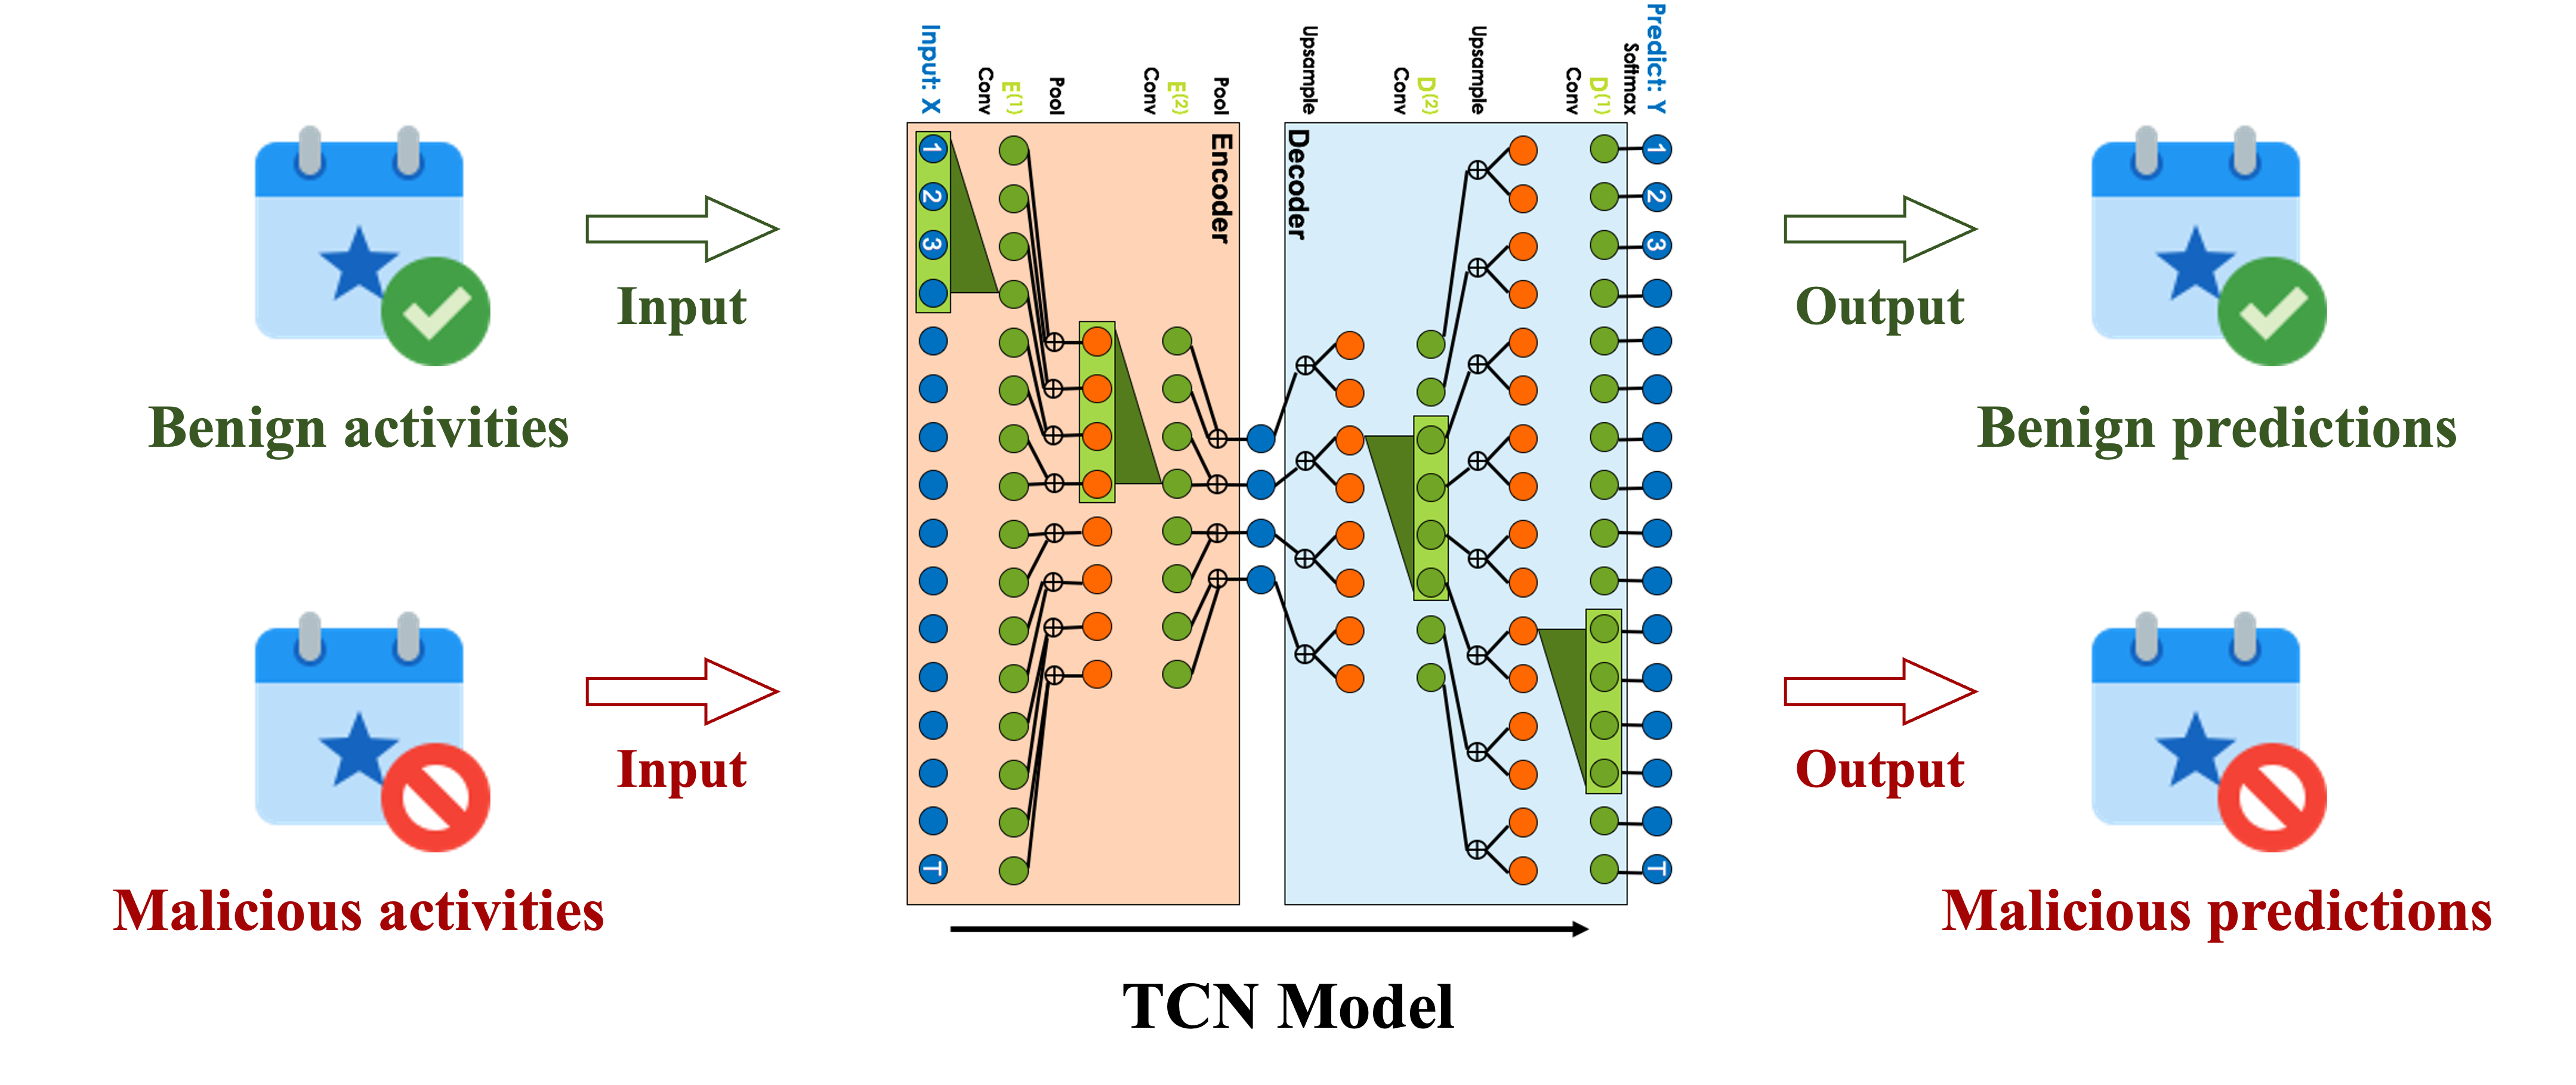
\includegraphics[width=1.00\linewidth]{FZU thesis templete//Fig/fig4-3.png}
    \caption{Operational mechanism of the temporal convolutional network.}
    \label{fig-4-2}
\end{figure}


% ————————————————————————————————————————————————————————————————————— %
% ————————————————————————————————————————————————————————————————————— %

\subsubsection{Classification Models}
\noindent Following the identification of suspicious data batches, the next step involves classifying these packets into two categories: benign or malicious. In this research, a text-convolutional neural network (text-CNN) \cite{min2018tr} is employed for the extraction of traffic features. Text-CNNs are specialized types of convolutional neural networks designed to handle text data. They apply convolutional layers to extract higher-level features from text data structured as input vectors, making them highly effective for tasks involving natural language processing and text analysis.

\vspace{8pt}

For packet classification, this project employs four cost-efficient classifiers: Support Vector Machine (SVM) \cite{ioannou2021network}, K-Nearest Neighbors (KNN) \cite{lahmadi2020mitm}, Random Forest (RF) \cite{min2018tr}, and Naïve Bayes \cite{mehmood2018nbc}. This multi-classifier approach helps to mitigate potential biases in text analysis by diversifying the analytical perspectives. Network payload-based features are generated by converting the payload bytes into low-dimensional vectors using \textit{Word2Vec} techniques, which effectively capture the semantic relationships within the data. These vectors form the input for the text-CNN, where key traffic features are extracted. The features extracted by the text-CNN are then concatenated with statistical features to create a comprehensive feature set for the final classification models.

\vspace{8pt}

The workflow for packet classification using text-CNN is illustrated in \textbf{Figure 4-3}, where it can be seen how raw data is transformed through various stages of processing to classify packets accurately as either benign or malicious.

\begin{figure} %[H]
    \centering
    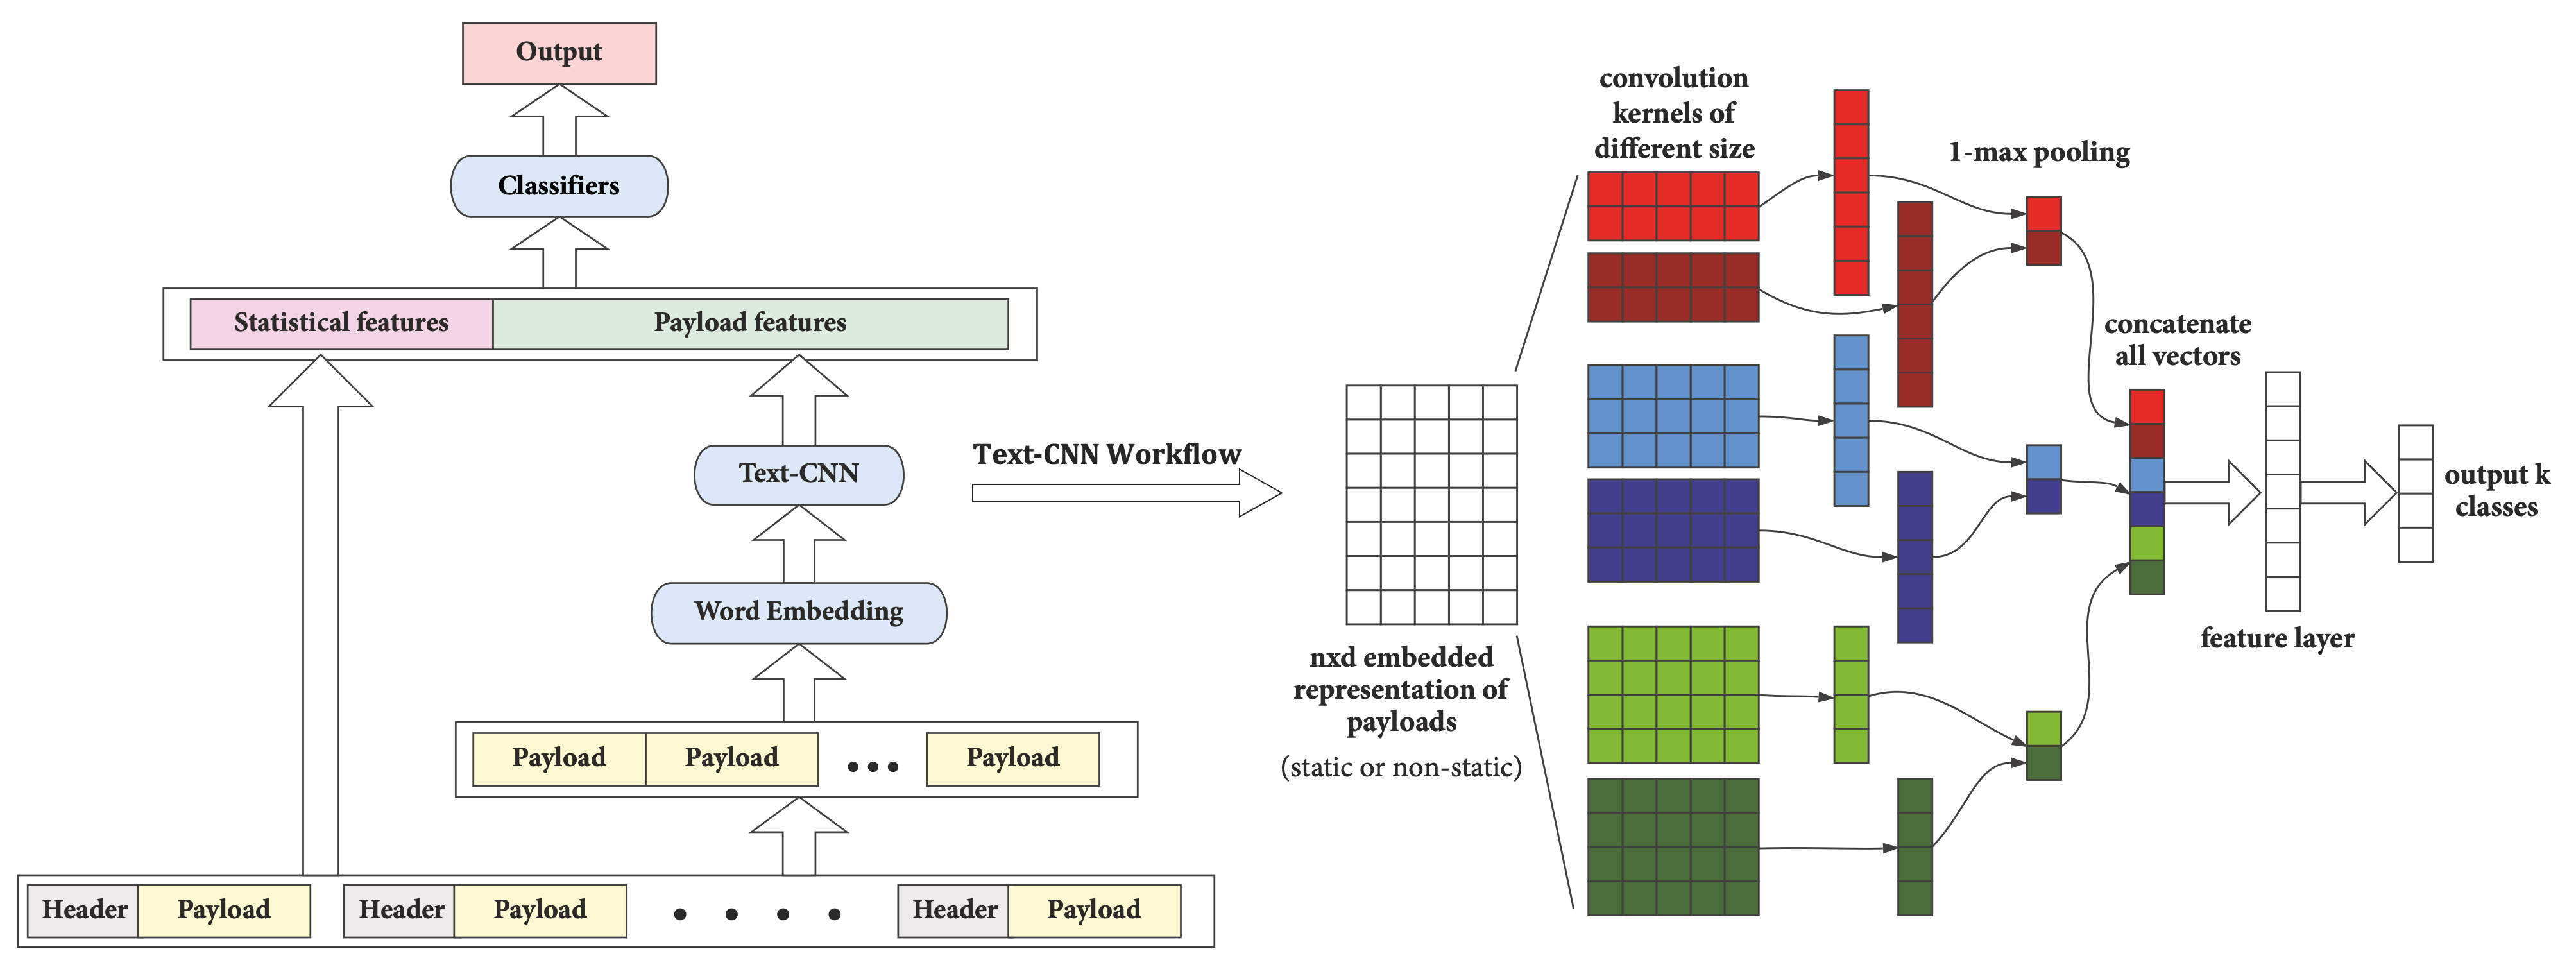
\includegraphics[width=1.00\linewidth]{FZU thesis templete//Fig/fig4-4.png}
    \caption{The general architecture of the classification models.}
    \label{fig-4-3}
\end{figure}

% ————————————————————————————————————————————————————————————————————— %
% ————————————————————————————————————————————————————————————————————— %

\subsubsection{System Overview}
\noindent BLEGuard is designed to optimize the balance between detection accuracy and power consumption. As depicted in \textbf{Figure 4-4}, the system employs a flexible approach where the pre-detection algorithm is utilized to maintain efficiency under GPU resource constraints, minimizing power and computational overhead. In scenarios where high detection accuracy is paramount, the reconstruction model is activated to enhance analytical precision. Moreover, the classification models within BLEGuard are adept at precisely identifying malicious advertising packets, providing targeted feedback that significantly augments the efficacy of the detection modules. This versatile framework ensures that BLEGuard can adapt to varying operational demands, thereby maintaining robust security measures without compromising on network performance.

\vspace{4pt}

\begin{figure}[H]
    \centering
    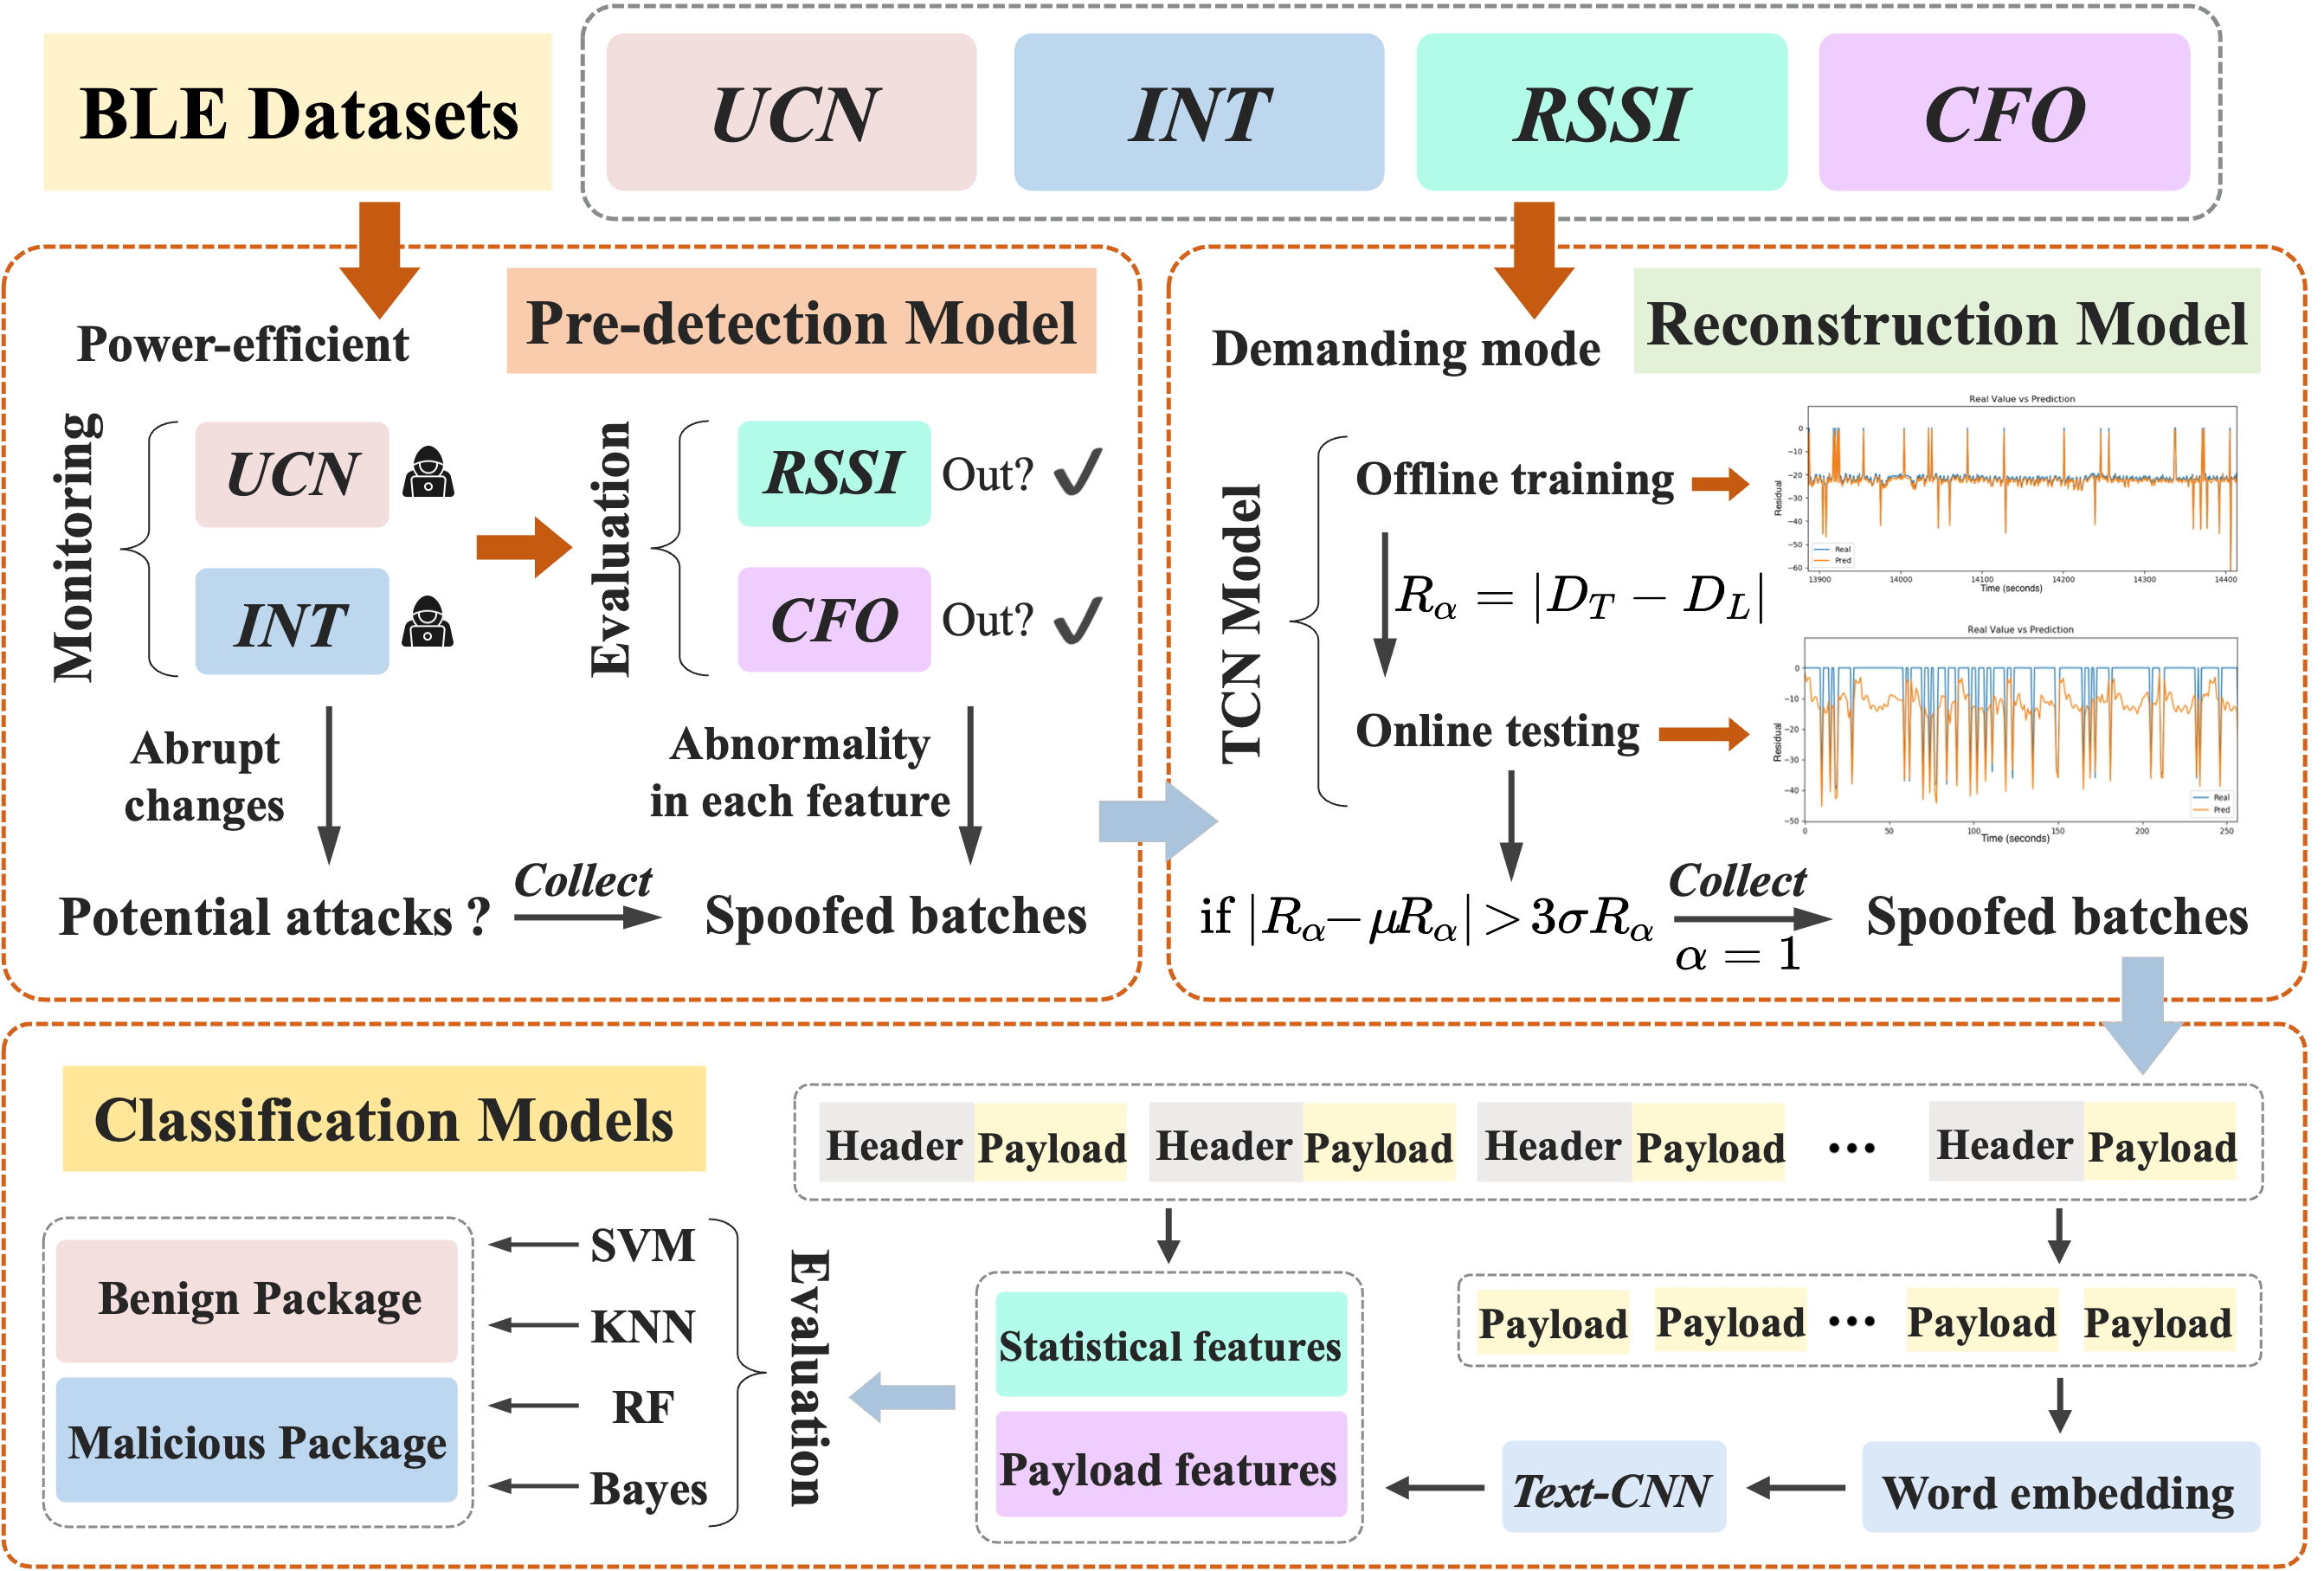
\includegraphics[width=0.92\linewidth]{FZU thesis templete//Fig/fig4-2.png}
    \caption{The overall workflow of \textit{BLEGuard} detection mechanism.}
    \label{fig-4-4}
\end{figure}

In this chapter, we have provided a comprehensive description of the construction process for the BLE-SAD dataset, as well as a detailed exposition of the mathematical models and operational mechanisms underpinning the BLEGuard System. The subsequent chapter will delve into the specific parameter settings of the models, as well as present the experimental data and results, demonstrating the effectiveness of BLEGuard in various testing scenarios.

\newpage